\documentclass[border=10pt]{standalone}

\usepackage{tikz}
\usepackage{tikzsymbols}
\usetikzlibrary{calc,patterns,shapes.geometric}

\def\centerarc[#1](#2)(#3:#4:#5){\draw[#1] ($(#2)+({#5*cos(#3)},{#5*sin(#3)})$) arc (#3:#4:#5);}

\begin{document}
	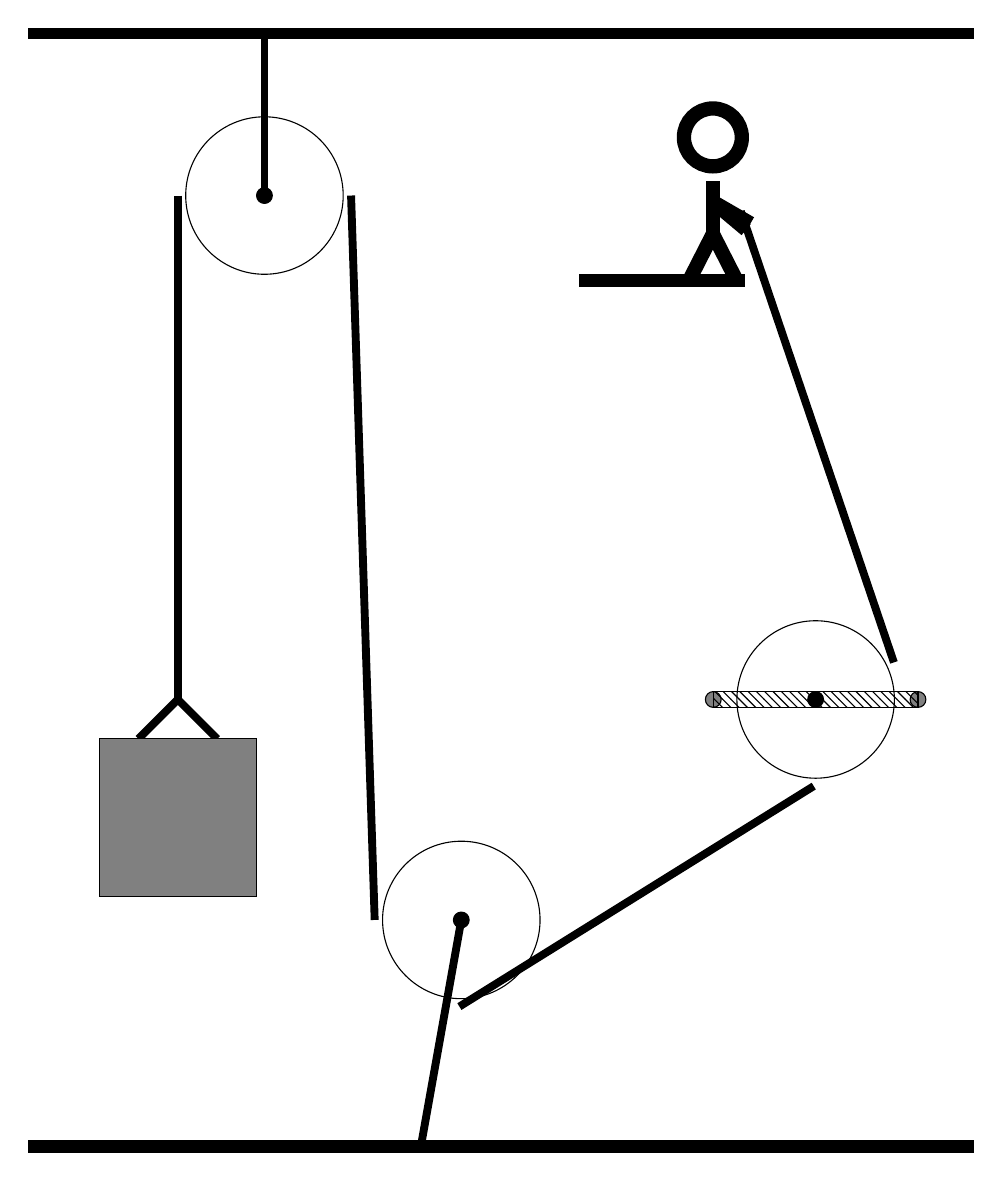
\begin{tikzpicture}
		%%%%% START %%%%%
		\draw[fill=black] (-2, 14) rectangle (10, 14.125);
		
		\draw (1, 12) circle (1);
		\draw[fill=black] (1, 12) circle (0.1);
		\draw[line width=1mm] (1, 14) -- (1, 12);
		
		\draw (3.5, 2.8) circle (1);
		\draw[fill=black] (3.5, 2.8) circle (0.1);
		\draw[line width=1mm] (3.5, 2.8) -- (3.0, 0);
		
		\draw[fill=white](8, 5.6) circle (1);
		\draw[fill=black] (8, 5.6) circle (0.1);
		\draw[fill=black!50] (9.3, 5.6) circle (0.1);
		\draw[fill=black!50] (6.7, 5.6) circle (0.1);
		\draw[pattern=north west lines, pattern color=black] (6.7, 5.7) rectangle (9.3, 5.5);
		
		\draw[line width=1mm](-0.6, 5.1) --  (-0.1, 5.6) -- (0.4, 5.1);
		\draw[fill=black!50] (-1.1, 5.1) rectangle (0.9, 3.1);
		
		\draw[line width=1mm](-0.1, 12) -- (-0.1, 5.6);
		\centerarc[line width=1mm](1, 12)(180:0:1.1)
		\draw[line width=1mm](2.1, 12) -- (2.4, 2.8);
		\centerarc[line width=1mm](3.5, 2.8)(180:300:1.1);
		\draw[line width=1mm](3.476, 1.7) -- (7.976, 4.5);
		\centerarc[line width=1mm](8, 5.6)(300:390:1.1);
		\draw[line width=1mm](8.994, 6.071) -- (7.05, 11.8);
		
		\node at (6.75, 12) {\Strichmaxerl[10][-220][-30]};
		\draw[fill=black] (5, 11) rectangle (7.1, 10.85);
		
		\draw[fill=black] (-2, 0) rectangle (10, -0.15);
		%%%%% END %%%%%
	\end{tikzpicture}
\end{document}